
\section{Working with GStreamer in Python}
\gs is an open-source multimedia framework that provides a pipeline-based architecture for creating and manipulating multimedia applications \cite{gstreamerGStreamerOpenSource}.
It offers a comprehensive set of libraries, plugins, and tools for handling various types of multimedia data, including audio, video, and streaming media.
On the \gls{jetson} platform, \gs can be used to levrage the \glspl{asic}, such as the \gls{h265} encoder \cite{nvidiaAcceleratedGStreamerJetson}.

Following is a description of the different approaches that were tested for using \gs in \py.


\subsection{Communicating with a Gst-Launch Pipeline}
The easiest way to use \gs is to use \code{gst-launch-1.0} from the terminal, a tool that builda and runs basic \gs pipelines from a pipeline description string \cite{Gstlaunch1}.
An extensive list of examples on how to use \code{gst-launch-1.0} for various purposes has been made by Adrian Lane and can be found on his GitHub \cite{laneGStreamerPipelineSamples2020}.

Initially \code{gst-launch-1.0} was used to create pipelines to compress the images to \gls{h265} video streams and \gls{jpeg} images.
Different approaches were tested for communicating with the generated pipeline from Python.

\subsubsection{Method 1: Regular and temporary files}
A very simple and naive way to communicate with the pipeline is to use files.
The imput images were saved to files and the pipeline was set up to read from that file.
The opposite was done to get the output images.
When using regular files this approach was slow and not very reliable.
Using \gls{tmpfs}, which makes it possible to store temporary files in \gls{ram} instead of on disk improved the performance, but it still felt like a very naive approach \cite{dickinsTmpfsLinuxKernel2010}.

\subsubsection{Method 2: Network protocols}
The first approach to transfer the images was to send and receive data over the network.
\gs has both a \gls{tcp} client source and \gls{tcp} server sink that can be used to pipe data to the pipeline as well as from the pipeline.
Using \gls{tcp} was easy to set up and worked quite well as the pipeline could run independently in one process while a server serving input data and a output data client could run anywhere else, even on another computer on the same network.
The server an client were implemented in Python using the \gls{asyncio} library.
Using \gls{udp} was also tested and appeared to perform equally well, but made it impossible to monitor weither the pipeline was running properly and if any client were actually receiving data.


\subsubsection{Method 3: STDIN and STDOUT}
Another approach was to use \gls{stdin} and \gls{stdout} to pipe data to and from the pipeline.
\gls{asyncio}.
This approach is very similar in nature as using files, as \gls{stdin} and \gls{stdout}, like almost everything else in Linux, are represented as files \cite{mckayWhatAreStdin2020}.
However this approach is more elegant as it does not require any files and designed for this exact purpose.
The \gs process was started using \gls{asyncio} to be able to read and write to \gls{stdin} and \gls{stdout} asynchronously.

\subsubsection{Parsing of JPEG bytestream}
Initially the data generated from \gs was piped through \code{stdout}.
The following binary \gls{regex} was used in to separate the images.
\begin{figure}[H]
    \centering
    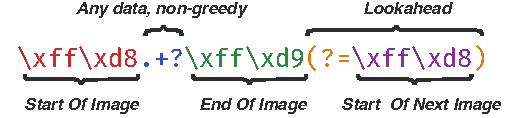
\includegraphics[width=0.7\textwidth]{figures/jpeg_regex.pdf}
\end{figure}
It looked for the beginning marker followed by data followed by the end marker and with a lookahead for the beginning marker of the next image.
The final lookahead was used to minimize the chance of parsing data bytes as the end marker as it was believed that could happen.
After analyzing the \gls{jpeg} standard however it was discovered that they use a technique called byte stuffing which ensures this never happens \cite[91]{ccittINFORMATIONTECHNOLOGYDIGITAL1992}.
Byte stuffing is a technique used in data transmission where special control characters are inserted into the data stream to distinguish between data and control information.
For \glspl{jpeg}, the zero byte is inserted after every control character that appears in the data \cite[91]{ccittINFORMATIONTECHNOLOGYDIGITAL1992}.
This made the parsing could be done both easier and faster by simply reading until the end-of-image marker.